% ============================================================
%  APPROACH / METHODOLOGY
% ============================================================
\section{Methodology}

This project aims to improve NanoChat by incorporating and evaluating several recent modelling
and training innovations. We begin by replicating the existing NanoChat codebase \parencite{nanochat}, which encompasses a GPT-2-style transformer architecture, a distributed training loop, and an evaluation harness.

We make the following four modifications below in isolation as a controlled experiment against the unmodified baseline, so that any performance change can be attributed to the specific technique.

\subsection{NanoChat Architecture}

NanoChat follows the GPT-2 decoder-only Transformer architecture with several modern refinements. The model consists of a stack of 12 Transformer blocks, each containing a Multi-Query Attention (MQA) sublayer followed by a Feed-Forward Network (FFN) with $\mathrm{ReLU}^2$ activation.
Each sublayer is preceded by RMSNorm and followed by a residual addition.
Input tokens are embedded via a learned embedding table and positional information is encoded
with rotary position embeddings (RoPE).
The model dimension is 768, with 12 attention heads of dimension 64, and the window pattern
\texttt{SSSL} (three sliding-window attention layers followed by one full-context layer) is
repeated across the depth.
The vocabulary is constructed using a custom Byte-Pair Encoder with UTF-8 byte fallback,
eliminating the need for an \texttt{<UNK>} token.
The final hidden state is projected to the vocabulary with a tied weight linear layer followed by a softmax.

\begin{figure}[h]
    \centering
    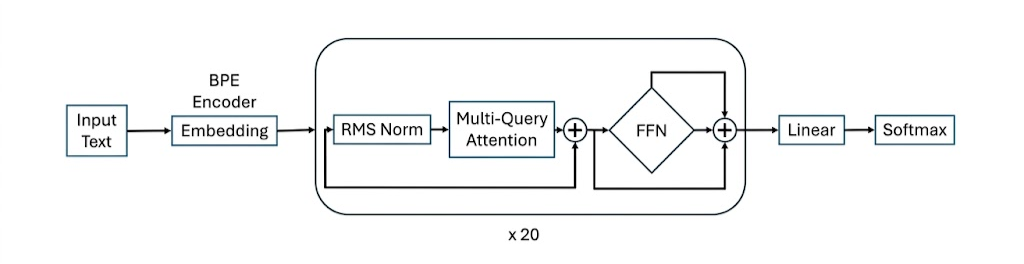
\includegraphics[width=1\textwidth]{images/nanochat_v2.png}
    \caption{Nanochat Architecture}
\end{figure}

\subsection{Experiment 1: Activation Functions}
The activation function shapes information flow and gradient dynamics in deep networks. ReLU \parencite{nair2010rectified} is the de-facto default for its simplicity and non-saturating gradient, but suffers from the ``dying ReLU'' problem. GeLU \parencite{hendrycks2016gelu} provides a smooth, probabilistically-motivated gating and has become dominant in large language models (GPT-2, BERT, and descendants). NanoChat instead adopts $\mathrm{ReLU}^2$, which improves sparsity and training efficiency in autoregressive models \parencite{so2021primer}.

More recently, \textcite{vitvitskyi2026mininggeneralizableactivationfunctions} used evolutionary search to discover activations that generalise across tasks, perturbing established functions with trigonometric components: \textit{GeLUSine} adds a sinusoidal correction to GeLU, while \textit{GELU-Sinc-Perturbation} (GSP) multiplicatively gates GeLU with a scaled sinc. These improved performance on vision benchmarks with small models, but their efficacy for language modelling was unestablished. Our experiments test this transfer, substituting the activation uniformly across all FFN sublayers. We evaluate six functions:
\begin{enumerate}\setlength{\itemsep}{1pt}\setlength{\parskip}{0pt}
    \item \textbf{ReLU\(^2\)} (baseline): $\mathrm{ReLU}^2(x) = \max(0,x)^2$.
    \item \textbf{GeLU} \parencite{hendrycks2016gelu}: $\mathrm{GeLU}(x) = \tfrac{x}{2}\!\left[1 + \mathrm{erf}(x/\sqrt{2})\right]$.
    \item \textbf{GeLUSine}: sinusoidal perturbation, $\mathrm{GeLUSine}(x) = \mathrm{GeLU}(x) + 0.1\sin x$.
    \item \textbf{GSP}: multiplicative sinc gate, $\mathrm{GSP}(x) = \mathrm{GeLU}(x)\!\left[1 + \tfrac{\alpha\sin(\pi x)}{\pi x}\right]$, with $\alpha{=}0.5$.
    \item \textbf{Gaussian-Modulated Tangent Unit (GMTU)}: a damped $\tanh$ with linear leak, $f(x) = \alpha\tanh(\beta x)\,e^{-\gamma x^2} + \lambda x$, with $\alpha{=}1.0,\beta{=}1.5,\gamma{=}0.2,\lambda{=}0.1$.
    \item \textbf{Turbulent}: a batch-wise activation adding a normalised sinusoidal perturbation to a log-scale base, $f(x_i) = \mathrm{sgn}(x_i)\ln(1+c|x_i|) + Ae^{-z_i^2/2}\sin(\omega x_i)$, where $z_i = (x_i - \mu_\mathcal{B})/(\sigma_\mathcal{B}+\epsilon)$ uses batch statistics, with $c{=}0.5,A{=}0.2,\omega{=}2.0,\epsilon{=}10^{-6}$.
\end{enumerate}

% \subsection{Experiment 1: Activation Functions}

% The choice of activation function has a significant effect on the information flow and gradient dynamics of deep networks.

% The Rectified Linear Unit (ReLU) \parencite{nair2010rectified} has become the de-facto default due to its simplicity and non-saturating gradient, though it suffers from the ``dying ReLU'' problem for negative inputs.

% \textcite{hendrycks2016gelu} proposed the Gaussian Error Linear Unit (GeLU), which provides a smooth, probabilistically-motivated gating of inputs. GeLU has since become the dominant activation in large language models including GPT-2, BERT, and their descendants.

% NanoChat adopts $\mathrm{ReLU}^2$ (applying ReLU twice), which has been shown to improve sparsity and training efficiency in autoregressive models \parencite{so2021primer}.

% %\begin{figure}[h]
% %    \centering
% %    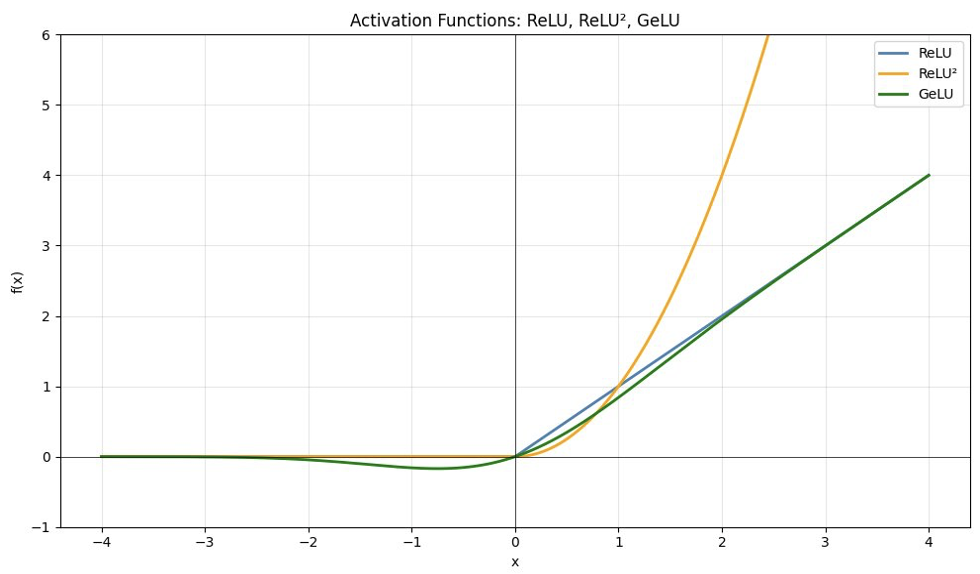
\includegraphics[width=0.67\textwidth]{images/activation.png}
% %\end{figure}

% More recently, \textcite{vitvitskyi2026mininggeneralizableactivationfunctions} applied
% evolutionary search to discover activation functions that generalise across tasks.
% Their approach perturbs established functions with trigonometric components: \textit{GeLUSine}
% adds a sinusoidal correction $0.1\sin(x)$ to GeLU, while \textit{GELU-Sinc-Perturbation} (GSP)
% multiplicatively gates GeLU with a scaled sinc function.
% These activations achieved improved performance on computer vision benchmarks with small models, though their efficacy for language modelling had not been established.

% Our experiments directly test this transfer. In all experiments, the activation function is substituted uniformly across all FFN sublayers.
% We evaluate the following six functions:

% \begin{enumerate}
%     \item \textbf{ReLU\(^2\)} (baseline): $\mathrm{ReLU}^2(x) = \max(0,x)^2$

%     \item \textbf{GeLU} \parencite{hendrycks2016gelu}:
%         \[\mathrm{GeLU}(x) = \frac{x}{2}\!\left[1 + \mathrm{erf}\!\left(\frac{x}{\sqrt{2}}\right)\right]\]

%     \item \textbf{GeLUSine}: a sinusoidal perturbation of GeLU,
%         \[\mathrm{GeLUSine}(x) = \mathrm{GeLU}(x) + 0.1\sin x\]

%     \item \textbf{GELU-Sinc-Perturbation (GSP)}: a multiplicative sinc gate applied to GeLU,
%         \[\mathrm{GSP}(x) = \mathrm{GeLU}(x)\!\left[1 + \alpha\cdot\mathrm{sinc}(x)\right]
%           = \mathrm{GeLU}(x)\!\left[1 + \frac{\alpha\sin(\pi x)}{\pi x}\right], \quad \alpha = 0.5\]

          

%     \item \textbf{Gaussian-Modulated Tangent Unit (GMTU)}: a custom activation combining a
%         damped hyperbolic tangent with a linear leak,
%         \[f(x) = \alpha\tanh(\beta x)\cdot e^{-\gamma x^2} + \lambda x,
%           \quad \alpha{=}1.0,\; \beta{=}1.5,\; \gamma{=}0.2,\; \lambda{=}0.1\]

%     \item \textbf{Turbulent}: a batch-wise activation that introduces a statistically-normalised
%         sinusoidal perturbation on top of a log-scale base,
%         \[f(\mathbf{x}) = \mathrm{sgn}(x_i)\ln(1+c|x_i|) + Ae^{-\frac{1}{2}z_i^2}\sin(\omega x_i),
%           \quad z_i = \frac{x_i - \mu_\mathcal{B}}{\sigma_\mathcal{B}+\epsilon}\]
%         where $\mu_\mathcal{B}$ and $\sigma_\mathcal{B}$ are the batch mean and standard
%         deviation, and $c{=}0.5$, $A{=}0.2$, $\omega{=}2.0$, $\epsilon{=}10^{-6}$.
% \end{enumerate}

\subsection{Experiment 2: Multi-Token Prediction Loss}

Standard next-token prediction trains the model to predict $x_{t+1}$ given the context
$x_{1:t}$. The standard next-token prediction objective is:
\begin{equation*}
    L_1 = -\sum_t \log P_\theta(x_{t+1} \mid x_{1:t})
\end{equation*}

While simple and effective, this one-step objective has been criticised for promoting
``lazy'' representations that exploit local statistics rather than longer-range structure, and is vulnerable to \emph{error avalanche}: small mistakes in generation propagate and compound over many steps.

\textcite{gloeckle2024better} proposed \textbf{Multi-Token Prediction (MTP)}, which trains
$n$ independent output heads to simultaneously predict the next $n$ tokens:
\begin{equation*}
    L_n = -\sum_t \log P_\theta(x_{t+1:t+n} \mid x_{1:t})
\end{equation*}

We experiment with $n=4$ prediction heads. MTP supposedly encourages the model to develop more structured internal representations, as the shared hidden state must support accurate prediction at multiple horizons simultaneously.

MTP also opens additional inference-time options such as speculative decoding. However, there is an overhead of $n$ output heads and the additional memory required to store intermediate
activations, which we we quantify in our experiments.

\subsection{Experiment 3: Engram Layer}

We integrate an \textbf{Engram layer} \parencite{cheng2026conditional} into the NanoChat
architecture while keeping total parameter count approximately fixed by reducing the depth of one standard transformer block.

The Engram layer augments specific transformer blocks with a differentiable key-value memory
store addressed by \(n\)-gram hash identifiers.
At each forward pass, the module (i) computes \(n\)-gram hash IDs from the input token sequence, module (ii) performs an $O(1)$ lookup to retrieve cached embeddings from the memory store, and module (iii) adds the retrieved vectors back into the hidden state via a learned gating mechanism before the standard transformer block.
Following the original paper's prescription for shallow models, we attach Engram modules to
layers 2 and 6 (out of 12), anticipating that these positions balance early contextual grounding with mid-depth feature enrichment.

\begin{figure}[H]
    \centering
    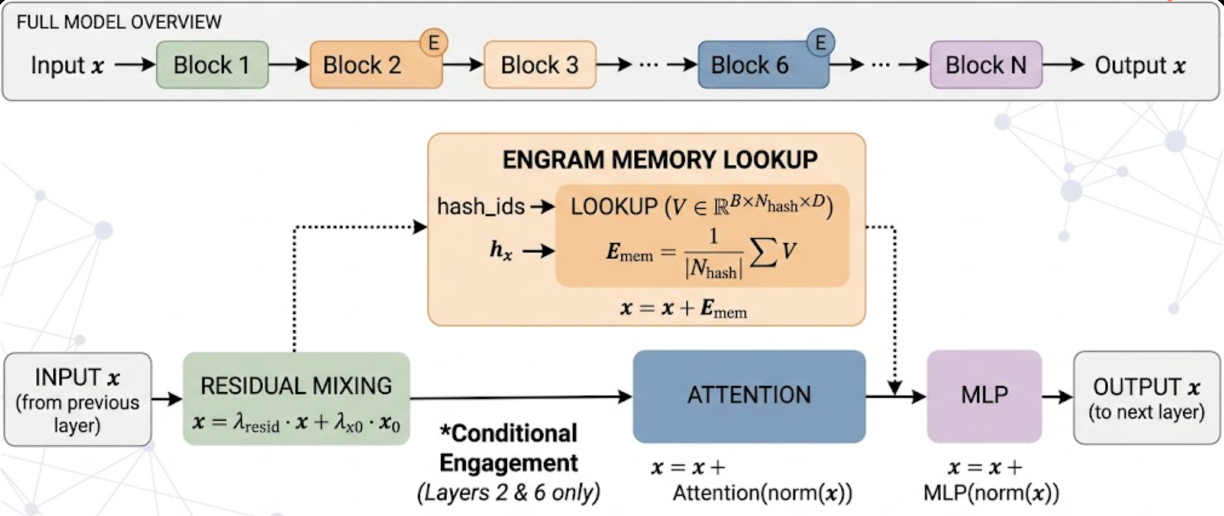
\includegraphics[width=0.8\textwidth]{images/engram_v2.png}
    \caption{Addition of Engram layer in Nanochat architecture}
\end{figure}

\subsection{Experiment 4: Attention Residuals}

Standard transformer residual connections apply a \emph{fixed, uniform} additive update at each
layer: $h_l = h_{l-1} + f_{l-1}(h_{l-1})$.
This causes uncontrolled growth in hidden-state magnitude with depth and progressively dilutes the
contribution of early layers \parencite{chen2026attnres}.
We replace this fixed accumulation with \textbf{Attention Residuals (AttnRes)}
\parencite{chen2026attnres}: each layer computes a learned softmax attention over all preceding
layer outputs, with a small learnable per-layer pseudo-query vector $w_l$.
Formally, let $\{h_0, h_1, \ldots, h_{l-1}\}$ denote the stored outputs of all preceding layers.
The AttnRes update is:
\begin{equation*}
    h_l = \sum_{i=0}^{l-1} \alpha_{i \to l}\, h_i + f_{l-1}(h_{l-1}),
    \quad \boldsymbol{\alpha} = \mathrm{softmax}(w_l^\top [h_0, \ldots, h_{l-1}])
\end{equation*}
For NanoChat's modest depth of 12 layers, Full AttnRes is computationally practical and we do not need to  employ the Block AttnRes variant.
The overhead is minimal, as the preceding layer outputs are already retained in memory during backpropagation.
